\subsubsection{A Cardboard Model}

A possible representation is a so called `carboard model', which is a set of interconnected planar patches used to represent human limbs. This is used in `Cardboard People: A Parameterized Model of Articulated Image Motion'\cite{cardboardpeople}, where S. Ju et al tracked a walking movement in two dimensions using two body parts - the thigh and the calf. These articulated components were governed by their `translation' and `curl' (that is rotation) in a side view of the walk. For more robust modelling from other camera angles, components could be governed by their `divergence', `deformation', `yaw' and `pitch'. The culmination of these parameters defines each cardboard segment's location in two-dimensional space, but compensates for three-dimensional movement of the subject. Figure~\ref{fig:cardboardmodel} shows an example model and the effects of adjustments of these parameters.

\begin{figure}[H]
    \centering
    \subfigure[A cardboard model]{
            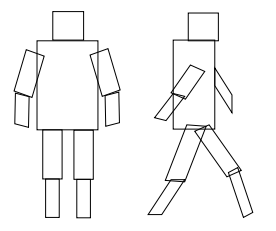
\includegraphics[height=6cm]{background/images/cardboard}
    }
    \subfigure[Parameters governing position of a cardboard segment]{
            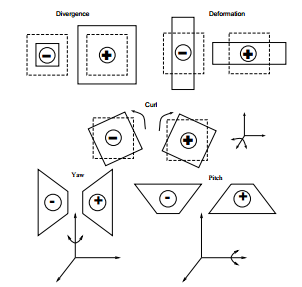
\includegraphics[height=6cm]{background/images/cardboard2}
    }
\caption{The cardboard model used by S. Ju et al\cite{cardboardpeople}}
\label{fig:cardboardmodel}
\end{figure}

Other similar primitive shape representations such as cylinders, ellipsoids and cones are often used\cite{cvmocapsurvey}.